%% bare_jrnl_compsoc.tex
%% V1.4b
%% 2015/08/26
%% by Michael Shell
%% See:
%% http://www.michaelshell.org/
%% for current contact information.
%%
%% This is a skeleton file demonstrating the use of IEEEtran.cls
%% (requires IEEEtran.cls version 1.8b or later) with an IEEE
%% Computer Society journal paper.
%%
%% Support sites:
%% http://www.michaelshell.org/tex/ieeetran/
%% http://www.ctan.org/pkg/ieeetran
%% and
%% http://www.ieee.org/

%%*************************************************************************
%% Legal Notice:
%% This code is offered as-is without any warranty either expressed or
%% implied; without even the implied warranty of MERCHANTABILITY or
%% FITNESS FOR A PARTICULAR PURPOSE! 
%% User assumes all risk.
%% In no event shall the IEEE or any contributor to this code be liable for
%% any damages or losses, including, but not limited to, incidental,
%% consequential, or any other damages, resulting from the use or misuse
%% of any information contained here.
%%
%% All comments are the opinions of their respective authors and are not
%% necessarily endorsed by the IEEE.
%%
%% This work is distributed under the LaTeX Project Public License (LPPL)
%% ( http://www.latex-project.org/ ) version 1.3, and may be freely used,
%% distributed and modified. A copy of the LPPL, version 1.3, is included
%% in the base LaTeX documentation of all distributions of LaTeX released
%% 2003/12/01 or later.
%% Retain all contribution notices and credits.
%% ** Modified files should be clearly indicated as such, including  **
%% ** renaming them and changing author support contact information. **
%%*************************************************************************


% *** Authors should verify (and, if needed, correct) their LaTeX system  ***
% *** with the testflow diagnostic prior to trusting their LaTeX platform ***
% *** with production work. The IEEE's font choices and paper sizes can   ***
% *** trigger bugs that do not appear when using other class files.       ***                          ***
% The testflow support page is at:
% http://www.michaelshell.org/tex/testflow/


\documentclass[10pt,journal,compsoc]{IEEEtran}
%
% If IEEEtran.cls has not been installed into the LaTeX system files,
% manually specify the path to it like:
% \documentclass[10pt,journal,compsoc]{../sty/IEEEtran}





% Some very useful LaTeX packages include:
% (uncomment the ones you want to load)


% *** MISC UTILITY PACKAGES ***
%
%\usepackage{ifpdf}
% Heiko Oberdiek's ifpdf.sty is very useful if you need conditional
% compilation based on whether the output is pdf or dvi.
% usage:
% \ifpdf
%   % pdf code
% \else
%   % dvi code
% \fi
% The latest version of ifpdf.sty can be obtained from:
% http://www.ctan.org/pkg/ifpdf
% Also, note that IEEEtran.cls V1.7 and later provides a builtin
% \ifCLASSINFOpdf conditional that works the same way.
% When switching from latex to pdflatex and vice-versa, the compiler may
% have to be run twice to clear warning/error messages.






% *** CITATION PACKAGES ***
%
\ifCLASSOPTIONcompsoc
  % IEEE Computer Society needs nocompress option
  % requires cite.sty v4.0 or later (November 2003)
  \usepackage[nocompress]{cite}
\else
  % normal IEEE
  \usepackage{cite}
\fi
% cite.sty was written by Donald Arseneau
% V1.6 and later of IEEEtran pre-defines the format of the cite.sty package
% \cite{} output to follow that of the IEEE. Loading the cite package will
% result in citation numbers being automatically sorted and properly
% "compressed/ranged". e.g., [1], [9], [2], [7], [5], [6] without using
% cite.sty will become [1], [2], [5]--[7], [9] using cite.sty. cite.sty's
% \cite will automatically add leading space, if needed. Use cite.sty's
% noadjust option (cite.sty V3.8 and later) if you want to turn this off
% such as if a citation ever needs to be enclosed in parenthesis.
% cite.sty is already installed on most LaTeX systems. Be sure and use
% version 5.0 (2009-03-20) and later if using hyperref.sty.
% The latest version can be obtained at:
% http://www.ctan.org/pkg/cite
% The documentation is contained in the cite.sty file itself.
%
% Note that some packages require special options to format as the Computer
% Society requires. In particular, Computer Society  papers do not use
% compressed citation ranges as is done in typical IEEE papers
% (e.g., [1]-[4]). Instead, they list every citation separately in order
% (e.g., [1], [2], [3], [4]). To get the latter we need to load the cite
% package with the nocompress option which is supported by cite.sty v4.0
% and later. Note also the use of a CLASSOPTION conditional provided by
% IEEEtran.cls V1.7 and later.





% *** GRAPHICS RELATED PACKAGES ***
%
\ifCLASSINFOpdf
  % \usepackage[pdftex]{graphicx}
  % declare the path(s) where your graphic files are
  % \graphicspath{{../pdf/}{../jpeg/}}
  % and their extensions so you won't have to specify these with
  % every instance of \includegraphics
  % \DeclareGraphicsExtensions{.pdf,.jpeg,.png}
\else
  % or other class option (dvipsone, dvipdf, if not using dvips). graphicx
  % will default to the driver specified in the system graphics.cfg if no
  % driver is specified.
  % \usepackage[dvips]{graphicx}
  % declare the path(s) where your graphic files are
  % \graphicspath{{../eps/}}
  % and their extensions so you won't have to specify these with
  % every instance of \includegraphics
  % \DeclareGraphicsExtensions{.eps}
\fi
% graphicx was written by David Carlisle and Sebastian Rahtz. It is
% required if you want graphics, photos, etc. graphicx.sty is already
% installed on most LaTeX systems. The latest version and documentation
% can be obtained at: 
% http://www.ctan.org/pkg/graphicx
% Another good source of documentation is "Using Imported Graphics in
% LaTeX2e" by Keith Reckdahl which can be found at:
% http://www.ctan.org/pkg/epslatex
%
% latex, and pdflatex in dvi mode, support graphics in encapsulated
% postscript (.eps) format. pdflatex in pdf mode supports graphics
% in .pdf, .jpeg, .png and .mps (metapost) formats. Users should ensure
% that all non-photo figures use a vector format (.eps, .pdf, .mps) and
% not a bitmapped formats (.jpeg, .png). The IEEE frowns on bitmapped formats
% which can result in "jaggedy"/blurry rendering of lines and letters as
% well as large increases in file sizes.
%
% You can find documentation about the pdfTeX application at:
% http://www.tug.org/applications/pdftex






% *** MATH PACKAGES ***
%
%\usepackage{amsmath}
% A popular package from the American Mathematical Society that provides
% many useful and powerful commands for dealing with mathematics.
%
% Note that the amsmath package sets \interdisplaylinepenalty to 10000
% thus preventing page breaks from occurring within multiline equations. Use:
%\interdisplaylinepenalty=2500
% after loading amsmath to restore such page breaks as IEEEtran.cls normally
% does. amsmath.sty is already installed on most LaTeX systems. The latest
% version and documentation can be obtained at:
% http://www.ctan.org/pkg/amsmath





% *** SPECIALIZED LIST PACKAGES ***
%
%\usepackage{algorithmic}
% algorithmic.sty was written by Peter Williams and Rogerio Brito.
% This package provides an algorithmic environment fo describing algorithms.
% You can use the algorithmic environment in-text or within a figure
% environment to provide for a floating algorithm. Do NOT use the algorithm
% floating environment provided by algorithm.sty (by the same authors) or
% algorithm2e.sty (by Christophe Fiorio) as the IEEE does not use dedicated
% algorithm float types and packages that provide these will not provide
% correct IEEE style captions. The latest version and documentation of
% algorithmic.sty can be obtained at:
% http://www.ctan.org/pkg/algorithms
% Also of interest may be the (relatively newer and more customizable)
% algorithmicx.sty package by Szasz Janos:
% http://www.ctan.org/pkg/algorithmicx




% *** ALIGNMENT PACKAGES ***
%
%\usepackage{array}
% Frank Mittelbach's and David Carlisle's array.sty patches and improves
% the standard LaTeX2e array and tabular environments to provide better
% appearance and additional user controls. As the default LaTeX2e table
% generation code is lacking to the point of almost being broken with
% respect to the quality of the end results, all users are strongly
% advised to use an enhanced (at the very least that provided by array.sty)
% set of table tools. array.sty is already installed on most systems. The
% latest version and documentation can be obtained at:
% http://www.ctan.org/pkg/array


% IEEEtran contains the IEEEeqnarray family of commands that can be used to
% generate multiline equations as well as matrices, tables, etc., of high
% quality.




% *** SUBFIGURE PACKAGES ***
%\ifCLASSOPTIONcompsoc
%  \usepackage[caption=false,font=footnotesize,labelfont=sf,textfont=sf]{subfig}
%\else
%  \usepackage[caption=false,font=footnotesize]{subfig}
%\fi
% subfig.sty, written by Steven Douglas Cochran, is the modern replacement
% for subfigure.sty, the latter of which is no longer maintained and is
% incompatible with some LaTeX packages including fixltx2e. However,
% subfig.sty requires and automatically loads Axel Sommerfeldt's caption.sty
% which will override IEEEtran.cls' handling of captions and this will result
% in non-IEEE style figure/table captions. To prevent this problem, be sure
% and invoke subfig.sty's "caption=false" package option (available since
% subfig.sty version 1.3, 2005/06/28) as this is will preserve IEEEtran.cls
% handling of captions.
% Note that the Computer Society format requires a sans serif font rather
% than the serif font used in traditional IEEE formatting and thus the need
% to invoke different subfig.sty package options depending on whether
% compsoc mode has been enabled.
%
% The latest version and documentation of subfig.sty can be obtained at:
% http://www.ctan.org/pkg/subfig




% *** FLOAT PACKAGES ***
%
%\usepackage{fixltx2e}
% fixltx2e, the successor to the earlier fix2col.sty, was written by
% Frank Mittelbach and David Carlisle. This package corrects a few problems
% in the LaTeX2e kernel, the most notable of which is that in current
% LaTeX2e releases, the ordering of single and double column floats is not
% guaranteed to be preserved. Thus, an unpatched LaTeX2e can allow a
% single column figure to be placed prior to an earlier double column
% figure.
% Be aware that LaTeX2e kernels dated 2015 and later have fixltx2e.sty's
% corrections already built into the system in which case a warning will
% be issued if an attempt is made to load fixltx2e.sty as it is no longer
% needed.
% The latest version and documentation can be found at:
% http://www.ctan.org/pkg/fixltx2e


%\usepackage{stfloats}
% stfloats.sty was written by Sigitas Tolusis. This package gives LaTeX2e
% the ability to do double column floats at the bottom of the page as well
% as the top. (e.g., "\begin{figure*}[!b]" is not normally possible in
% LaTeX2e). It also provides a command:
%\fnbelowfloat
% to enable the placement of footnotes below bottom floats (the standard
% LaTeX2e kernel puts them above bottom floats). This is an invasive package
% which rewrites many portions of the LaTeX2e float routines. It may not work
% with other packages that modify the LaTeX2e float routines. The latest
% version and documentation can be obtained at:
% http://www.ctan.org/pkg/stfloats
% Do not use the stfloats baselinefloat ability as the IEEE does not allow
% \baselineskip to stretch. Authors submitting work to the IEEE should note
% that the IEEE rarely uses double column equations and that authors should try
% to avoid such use. Do not be tempted to use the cuted.sty or midfloat.sty
% packages (also by Sigitas Tolusis) as the IEEE does not format its papers in
% such ways.
% Do not attempt to use stfloats with fixltx2e as they are incompatible.
% Instead, use Morten Hogholm'a dblfloatfix which combines the features
% of both fixltx2e and stfloats:
%
% \usepackage{dblfloatfix}
% The latest version can be found at:
% http://www.ctan.org/pkg/dblfloatfix




%\ifCLASSOPTIONcaptionsoff
%  \usepackage[nomarkers]{endfloat}
% \let\MYoriglatexcaption\caption
% \renewcommand{\caption}[2][\relax]{\MYoriglatexcaption[#2]{#2}}
%\fi
% endfloat.sty was written by James Darrell McCauley, Jeff Goldberg and 
% Axel Sommerfeldt. This package may be useful when used in conjunction with 
% IEEEtran.cls'  captionsoff option. Some IEEE journals/societies require that
% submissions have lists of figures/tables at the end of the paper and that
% figures/tables without any captions are placed on a page by themselves at
% the end of the document. If needed, the draftcls IEEEtran class option or
% \CLASSINPUTbaselinestretch interface can be used to increase the line
% spacing as well. Be sure and use the nomarkers option of endfloat to
% prevent endfloat from "marking" where the figures would have been placed
% in the text. The two hack lines of code above are a slight modification of
% that suggested by in the endfloat docs (section 8.4.1) to ensure that
% the full captions always appear in the list of figures/tables - even if
% the user used the short optional argument of \caption[]{}.
% IEEE papers do not typically make use of \caption[]'s optional argument,
% so this should not be an issue. A similar trick can be used to disable
% captions of packages such as subfig.sty that lack options to turn off
% the subcaptions:
% For subfig.sty:
% \let\MYorigsubfloat\subfloat
% \renewcommand{\subfloat}[2][\relax]{\MYorigsubfloat[]{#2}}
% However, the above trick will not work if both optional arguments of
% the \subfloat command are used. Furthermore, there needs to be a
% description of each subfigure *somewhere* and endfloat does not add
% subfigure captions to its list of figures. Thus, the best approach is to
% avoid the use of subfigure captions (many IEEE journals avoid them anyway)
% and instead reference/explain all the subfigures within the main caption.
% The latest version of endfloat.sty and its documentation can obtained at:
% http://www.ctan.org/pkg/endfloat
%
% The IEEEtran \ifCLASSOPTIONcaptionsoff conditional can also be used
% later in the document, say, to conditionally put the References on a 
% page by themselves.

% *** PDF, URL AND HYPERLINK PACKAGES ***
%
%\usepackage{url}
% url.sty was written by Donald Arseneau. It provides better support for
% handling and breaking URLs. url.sty is already installed on most LaTeX
% systems. The latest version and documentation can be obtained at:
% http://www.ctan.org/pkg/url
% Basically, \url{my_url_here}.


% *** Do not adjust lengths that control margins, column widths, etc. ***
% *** Do not use packages that alter fonts (such as pslatex).         ***
% There should be no need to do such things with IEEEtran.cls V1.6 and later.
% (Unless specifically asked to do so by the journal or conference you plan
% to submit to, of course. )

% correct bad hyphenation here
\hyphenation{op-tical net-works semi-conduc-tor}

% Students may declare other LaTeX packages here
\usepackage{lipsum}
\usepackage{graphicx}
\usepackage{url}
\usepackage{hyperref}
\usepackage{tabularx}
\renewcommand{\arraystretch}{1.5}

\begin{document}


% ---- BUILT-IN DECLARATION OF ORIGINIALITY FORM  ----
\onecolumn
\thispagestyle{empty}  % No page number on the first page

\begin{center}
    {\LARGE \textbf{Declaration of Originality}}\\ \vspace{1cm}
    
    {\Large Unit Name: Advanced Artificial Intelligence Research Topics COMP6011}\\ \vspace{1cm}
    
\end{center}

    \textbf{I/We declare that:}
    \begin{itemize}
        \item The above information is complete and accurate.
        \item The work I am/We are submitting is entirely my/our own, except where clearly indicated otherwise and correctly referenced.
        \item I/We have taken (and will continue to take) all reasonable steps to ensure my/our work is not accessible to any other students who may gain unfair advantage from it.
        \item I/We have not previously submitted this work for any other unit, whether at Curtin University or elsewhere, or for prior attempts at this unit, except where clearly indicated otherwise.
    \end{itemize}

    \textbf{I/We understand that:}
    \begin{itemize}
        \item Plagiarism and collusion are dishonest and unfair to all other students.
        \item Detection of plagiarism and collusion may be done manually or by using tools (such as Turnitin).
        \item If I/We plagiarise or collude, I/We risk failing the unit with a grade of ANN (“Result Annulled due to Academic Misconduct”), which will remain permanently on my academic record. I/We also risk termination from my/our course and other penalties.
        \item Even with correct referencing, my/our submission will only be marked according to what I/we have done myself/ourselves, specifically for this assessment. I/We cannot re-use the work of others, or my/our own previously submitted work, in order to fulfil the assessment requirements.
        \item It is my/our responsibility to ensure that the submission is complete, correct, and not corrupted.
    \end{itemize}

    \textbf{I/We further declare that:}
 \begin{itemize}
    \item I/We have disclosed the use of any Generative Artificial Intelligence (GenAI) tools in the preparation of this assignment.
    \item Where GenAI tools were used, I/We have clearly stated:
    %%%%%%%%%%%%%%%%%%%%%%%%%%%%%%%%%%%%%%%%%%%%%%%%%%%%%%%%%%%%%%%%%%%%%%%%%%%%
    % Students to detail their use of GenAI below    
    \begin{itemize}
        \item the name(s) of the tool(s) used (e.g., ChatGPT, Copilot), and
        \item the extent and purpose of their use (e.g., brainstorming, language refinement, code assistance).
    \end{itemize}
    %%%%%%%%%%%%%%%%%%%%%%%%%%%%%%%%%%%%%%%%%%%%%%%%%%%%%%%%%%%%%%%%%%%%%%%%%%%%
    \item I/We confirm that all intellectual content, critical analysis, technical decisions, and conclusions remain my/our own work.
    \item I/We understand that undisclosed or inappropriate use of GenAI tools may constitute academic misconduct.
\end{itemize}

\textbf{Date:} {\today}

\begin{table}[h]
    \renewcommand{\arraystretch}{2}  % Adjusts row height for better readability
    \centering
    \begin{tabularx}{\textwidth}{|X|X|X|X|}
        \hline
        \textbf{Surname} & \textbf{Given Names} & \textbf{Student ID} & \textbf{Signature} \\ \hline
        Tandukar & Prasanna & 23047514 & 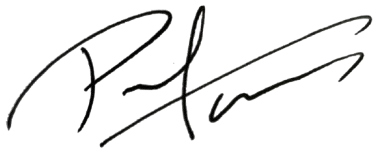
\includegraphics[height=1em]{signature.png} \\ \hline
       % & & & \\ \hline
       % & & & \\ \hline
       % & & & \\ \hline
    \end{tabularx}
\end{table}


\clearpage 
\twocolumn

% -------------------------------------------------------- 




\title{REPORT 1: TOPIC 1}

\author{Prasanna Tandukar,~\IEEEmembership{Master of Computing, 23047514}        % <-this % stops a space
\IEEEcompsocitemizethanks{\IEEEcompsocthanksitem Prasanna Tandukar is a Master of Computing, AI Major at Curtin University.\protect\\
% note need leading \protect in front of \\ to get a newline within \thanks as
% \\ is fragile and will error, could use \hfil\break instead.
E-mail: 23047514@student.curtin.edu.au\protect\\
}% <-this % stops an unwanted space
\thanks{Report started March 1; submitted April 4.}}

% The paper headers
\markboth{COMP6011 Advanced AI Research Topics}%
{Prasanna Tandukar, 23047514}

\IEEEtitleabstractindextext{%
\begin{abstract}
The importance of safer and efficient road freight transport has driven the development of advanced driver assistance systems (ADAS). Semantic segmentation is an important part of this system. This study evaluation various segmentation models for vehicle perception like FCN, DeepLabV3, and SegFormer. A combined method of literature review and benchmarking was utilized for practical application feasibility. Sample images from Cityscapes and BDD100K datasets were utilized. The models were compared with each other in areas of performance and computational efficiency. Results showed that FCN provided a basic baseline, DeepLabV3 improved accuracy but at a higher computational cost and SegFormer had the best balance between performance and speed. These findings show the effectiveness of transformer based models for real time ADAS systems and their potential for improve safety and reliability in freight transport systems.
\end{abstract}

% Note that keywords are not normally used for peerreview papers.
\begin{IEEEkeywords}
Computer Society, IEEE, IEEEtran, journal, \LaTeX, paper, template.
\end{IEEEkeywords}}


% make the title area
\maketitle

\IEEEdisplaynontitleabstractindextext




\IEEEraisesectionheading{\section{Introduction}\label{sec:introduction}}
\IEEEPARstart{T}{he} road freight sector in Australia is growing at a high pace due to high demand for goods and services within and outside the country \cite{Peters2023}. It also plays a massive role in Australia's national supply chain due to large geographical size and dispersed population \cite{BITRE2023}. Road freight is the most popular mode of transportation in Australia for transporting agricultural products, mining output and retail goods \cite{BITRE2023}. One of the main reasons for its dominance is due to its flexibility and accessibility. For example, it can provide door to door delivery connecting regional areas that does not have other modes of freight like rail or sea transport \cite{BITRE2023}. Major industries like agriculture, mining, construction, and retail heavily depends on road freight \cite{BITRE2023}.

There are numerous problems that current road freight in Australia faces including high rate of heavy vehicle crashes, driver fatigue, wildlife collisions and growing freight demand. Around 15--20\% of all road fatalities in Australia are caused by heavy vehicle crashes \cite{bitre_safety_statistics}. Instead of truck drivers, people of other vehicles who crashed with the truck accounted for about 75\% of total heavy truck fatalities\cite{bitre_safety_statistics}. Driver fatigue is also another major concern in road freight which can increase road accidents \cite{CASEY2024136} . This is caused due to long working hours, irregular schedules, lack of sleep and night driving \cite{CASEY2024136}.

Recent breakthroughs in artificial intelligence and computer vision have made it possible for the development of technologies such as advanced driver assistance systems (ADAS) \cite{s24196223}. This technology can help heavy truck drivers become more aware of their environment and it can minimize the possibility of accidents \cite{s24196223}. ADAS systems utilizes perception modules which analyzes visual data from the camera mounted in heavy trucks to understand the environment around it. By identifying various objects such as vehicles, pedestrians, road lanes, and traffic signs in its surroundings, perception system can provide important information to help in safe driving, navigation and decision making.

Semantic segmentation is one of the most popular and effective techniques for scene understanding in modern computer vision \cite{Long_2015_CVPR, garciagarcia2017reviewdeeplearningtechniques}. In contrast to other object detection techniques that uses boundary boxes, semantic segmentation uses a class label to every pixel in an image \cite{he2018maskrcnn}. This technique will helps the software system to identify various components of the driving environment like road surfaces, sidewalks, vehicles, cyclists, obstacles, etc. Such extreme detailed understanding of the environment is needed for the self driving systems to operate in complex road environments.

The aim of this research paper is to find the potential of semantic segmentation techniques in developing an effective perception module for heavy freight vehicles. This study focuses on both tradition and modern deep learning techniques for semantic segmentation. These techniques are analyzed and compared using publicly available autonomous driving datasets.

\section{Literature Review}
Semantic segmentation involves labeling each individual pixel in an image with a semantic label. It provides an output mask image where  pixel value represents different components in a scene such as road, sidewalk, vehicles, pedestrians, and signs. In road scene perception tasks, this is very important because it can be used to perform geometric reasoning, locate boundaries precisely, and process objects that are partially obstructed in an image \cite{Cordts_2016_CVPR}. This paper uses Cityscapes as a primary benchmark tool because it is considered as a standard benchmark tool for semantic urban scene understanding. It enables testing for high resolution street scene labeling and Intersection over Union (IoU) class metrics \cite{Cordts_2016_CVPR}. This dataset is also useful for testing issues on down-sampling for small objects which is useful for long range trucks as a pedestrian or cyclist in an image will only be few pixels big \cite{Cordts_2016_CVPR}.

\subsection{Classical Semantic Segmentation}
Traditional Semantic Segmentation techniques involved manual processes. Hand crafted feature sets were needed to give the computer specific instructions on what to look for like color, textures or edge patterns. TextonBoost is a classical semantic segmentation algorithm that uses texture based features called textons, along with boosting which is a machine learning technique \cite{Shotton2009}. TextonBoost to achieved simultaneous recognition and segmentation of objects in image scenes \cite{Shotton2009}. Other optimization based technique called graph cuts were also utilized for image segmentation. This method was capable of balancing region consistency with boundary smoothness to achieve globally optimal solutions for image segmentation \cite{937505}. Furthermore, probabilistic graphical models were utilized to achieve improvements in image segmentation quality through conditional random fields (CRF) \cite{krahenbuhl2012efficientinferencefullyconnected}. The development of dense CRF techniques allowed for fully connected pairwise pixel interactions through efficient approximate inference techniques \cite{krahenbuhl2012efficientinferencefullyconnected}. There was also superpixel algorithms like SLIC which reduced computational complexity through the partitioning of images into local coherent regions \cite{6205760}. This allowed for the transformation of pixel-level classification into region-level classification for image segmentation \cite{6205760}.

Although these methods sound impressive, it struggles in real world scenario. Firstly, these methods heavily rely on hand-engineered features (like edges, texture, color). If lighting conditions like day and night or weather conditions like rain and fog are different, or if sensor quality is low, then the model’s accuracy decreases significantly \cite{Shotton2009}. It is also not very effective in understanding the entire details in an image. In a road, there are large objects like road and sky and very small objects like traffic lights and pedestrians. Classical methods are not very effective in understanding both large and small objects at the same time \cite{Cordts_2016_CVPR}. Also, techniques like CRF has tendency to over smooth segmentation which can result in poor segmentation of smaller objects in an image \cite{Cordts_2016_CVPR}.

\begin{figure}[!t]
\centering
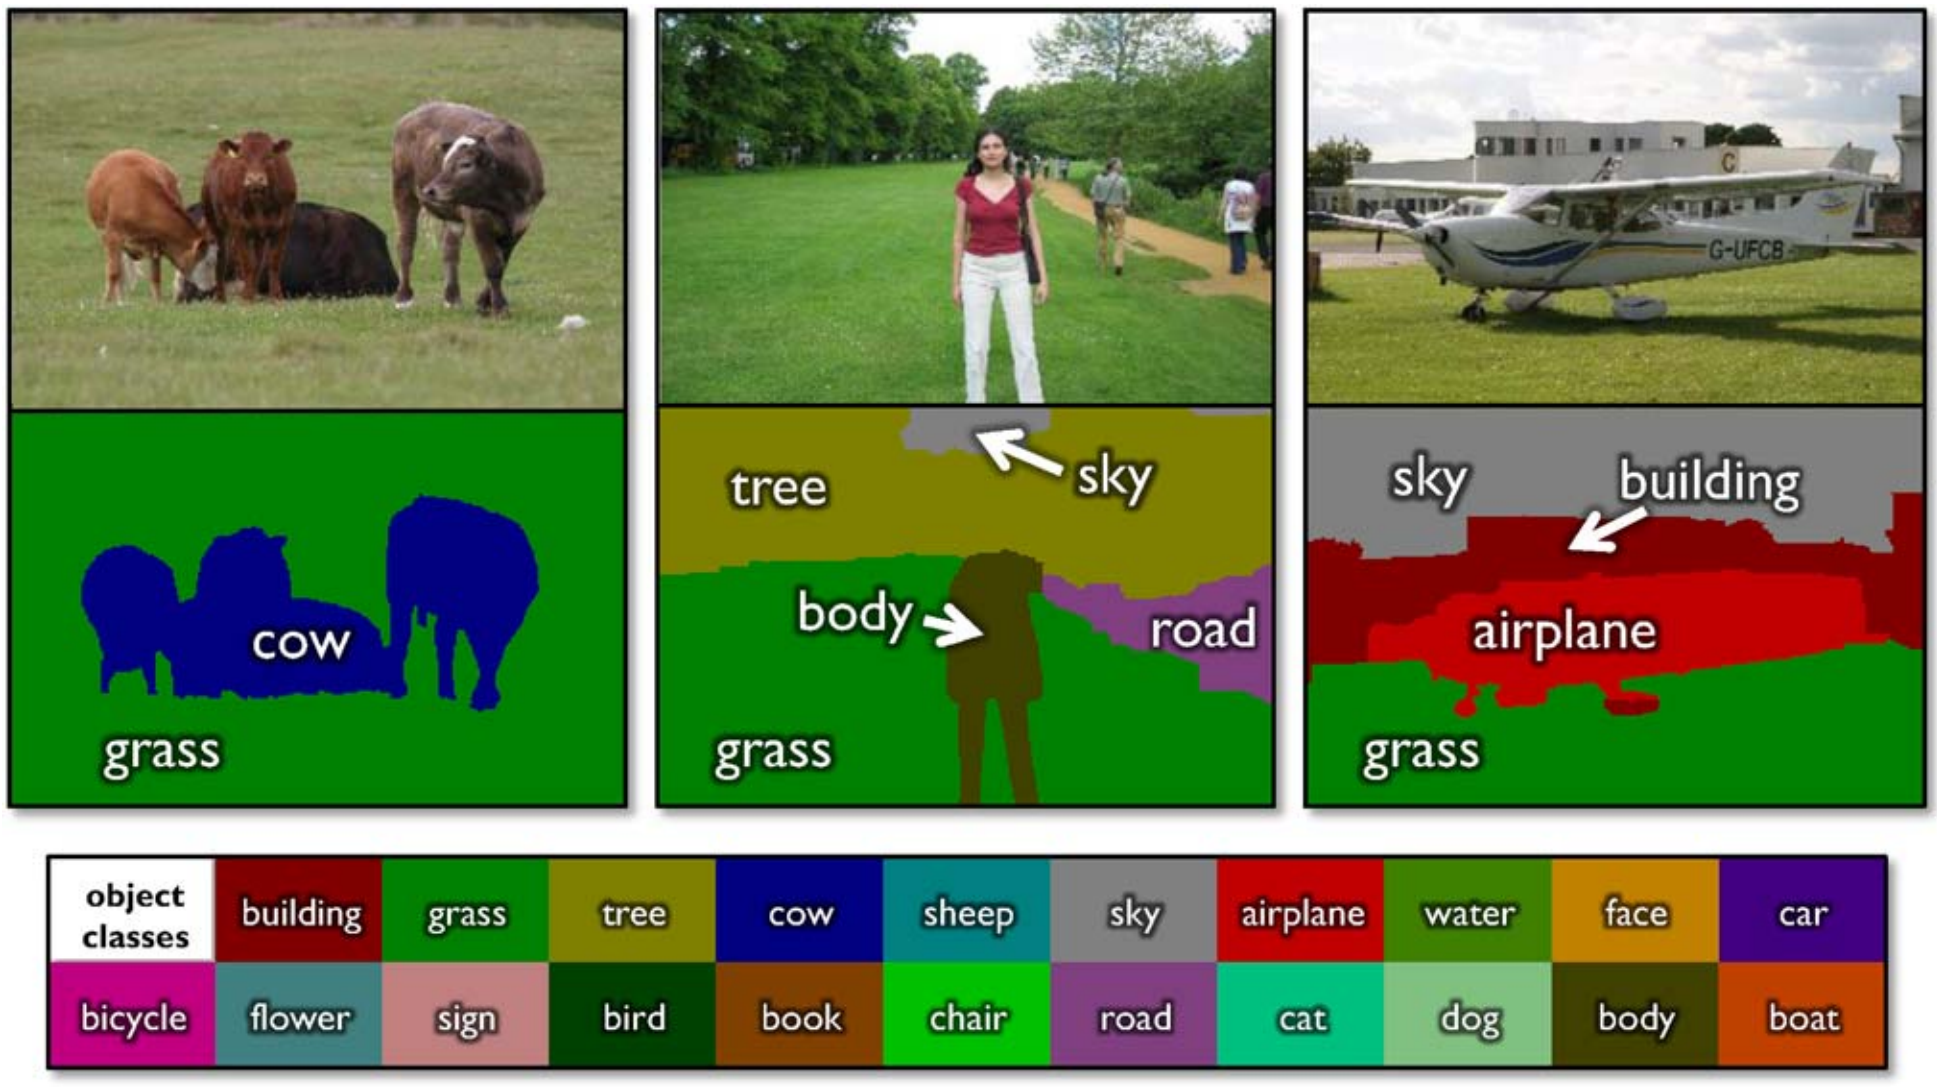
\includegraphics[width=\linewidth]{figs/textonboost.png}
% where an .eps filename suffix will be assumed under latex, 
% and a .pdf suffix will be assumed for pdflatex; or what has been declared
% via \DeclareGraphicsExtensions.
\caption{Example of simultaneous object recognition and semantic segmentation using the TextonBoost framework \cite{Shotton2009}.}
\label{fig:textonboost}
\end{figure}

\subsection{Deep Learning Segmentation}
\subsubsection{Fully Convolutional Networks (FCN)}
Fully Convolution Network is one of the deep learning segmentation methods utilizing concepts of convolution neural networks. It has led to significant advancements in segmentation techniques. FCNs replaces the original fully connected layers with convolutional layers \cite{long2015fullyconvolutionalnetworkssemantic}. While a normal CNN has a single label class for entire image, FCNs have labels for each individual pixels in an image \cite{long2015fullyconvolutionalnetworkssemantic}. This allows the network to operate in pixel wise prediction. The FCN architecture is based on the encoder-decoder network where the encoder is responsible for obtaining hierarchical semantic representations, while the decoder is responsible for progressively upsampling the obtained representations to their original resolution \cite{long2015fullyconvolutionalnetworkssemantic}. One of the major contributions made by FCNs is the use of skip connections, where the semantic representations obtained from the deeper layers are combined with the low-level spatial information obtained from the earlier layers \cite{long2015fullyconvolutionalnetworkssemantic}. In practical, ResNet is used in combination with FCNs to maintain the spatial resolution and increase the receptive field \cite{long2015fullyconvolutionalnetworkssemantic}. FCN is one of the efficient architectures that have shown good results on popular benchmarks like the Cityscapes dataset which this report uses. However, FCN architectures are not effective in obtaining accurate results in scenarios like lane boundary detection and free space estimation \cite{long2015fullyconvolutionalnetworkssemantic}.

\subsubsection{U-Net}
U-Net is a type of convolution neural network designed for semantic segmentation primarily for biomedical images \cite{ronneberger2015unetconvolutionalnetworksbiomedical}. But it was later applied for general images. The benefit of this architecture is that it gives good accuracy on small sample size of images \cite{ronneberger2015unetconvolutionalnetworksbiomedical}. Biomedical images with its labeled masks are difficult to find in large amount, so this architecture works with smaller number of input sample images. It is based on a symmetric encoder-decoder structure where the encoder extracts high-level semantic features with a series of downsampling operations \cite{ronneberger2015unetconvolutionalnetworksbiomedical}. The decoder then uses upsampling to reverse this and obtain spatial resolution \cite{ronneberger2015unetconvolutionalnetworksbiomedical}. One of the main feature of U-Net is that it heavily uses skip connections between encoder decoder layers \cite{ronneberger2015unetconvolutionalnetworksbiomedical}.

\begin{figure}[!t]
\centering
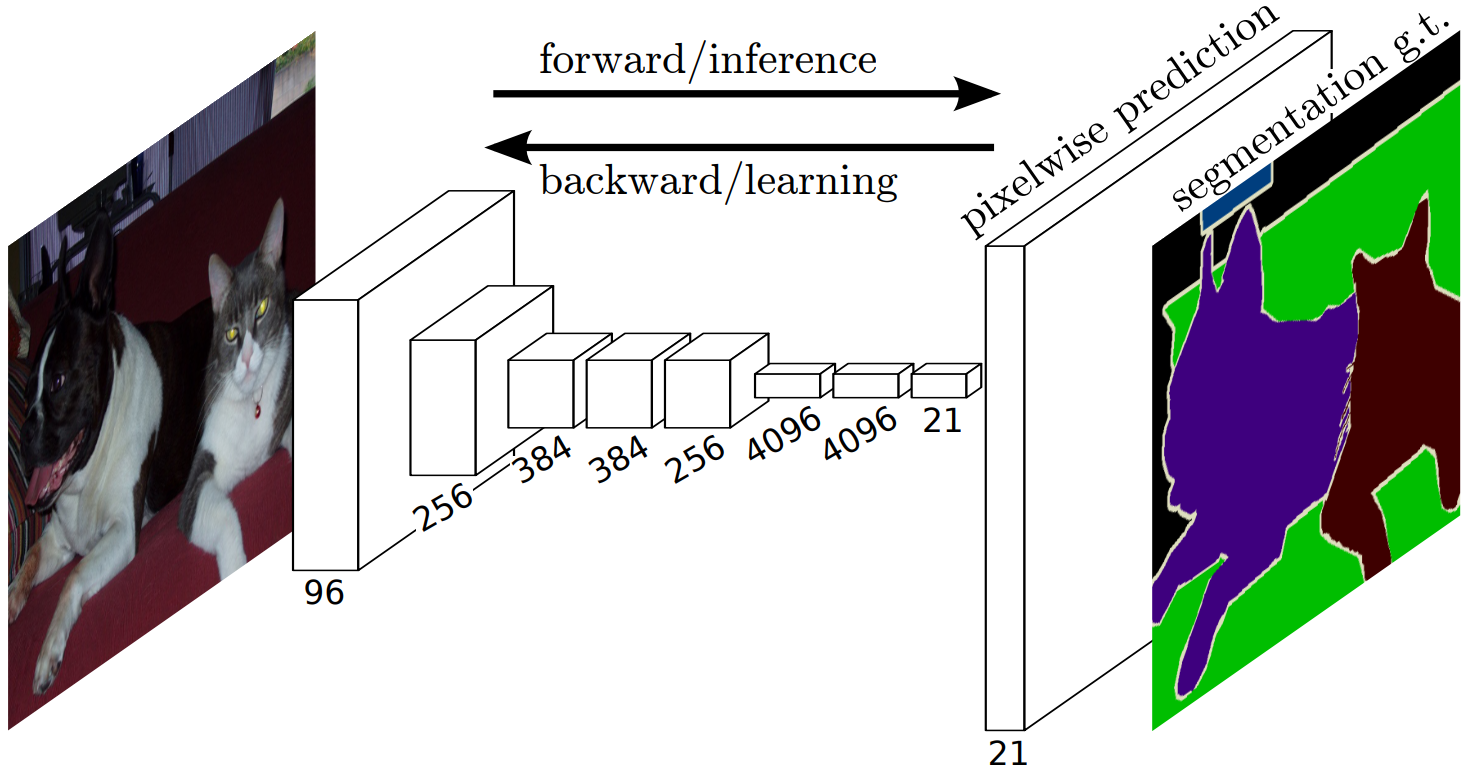
\includegraphics[width=0.48\columnwidth]{figs/fcn.png}
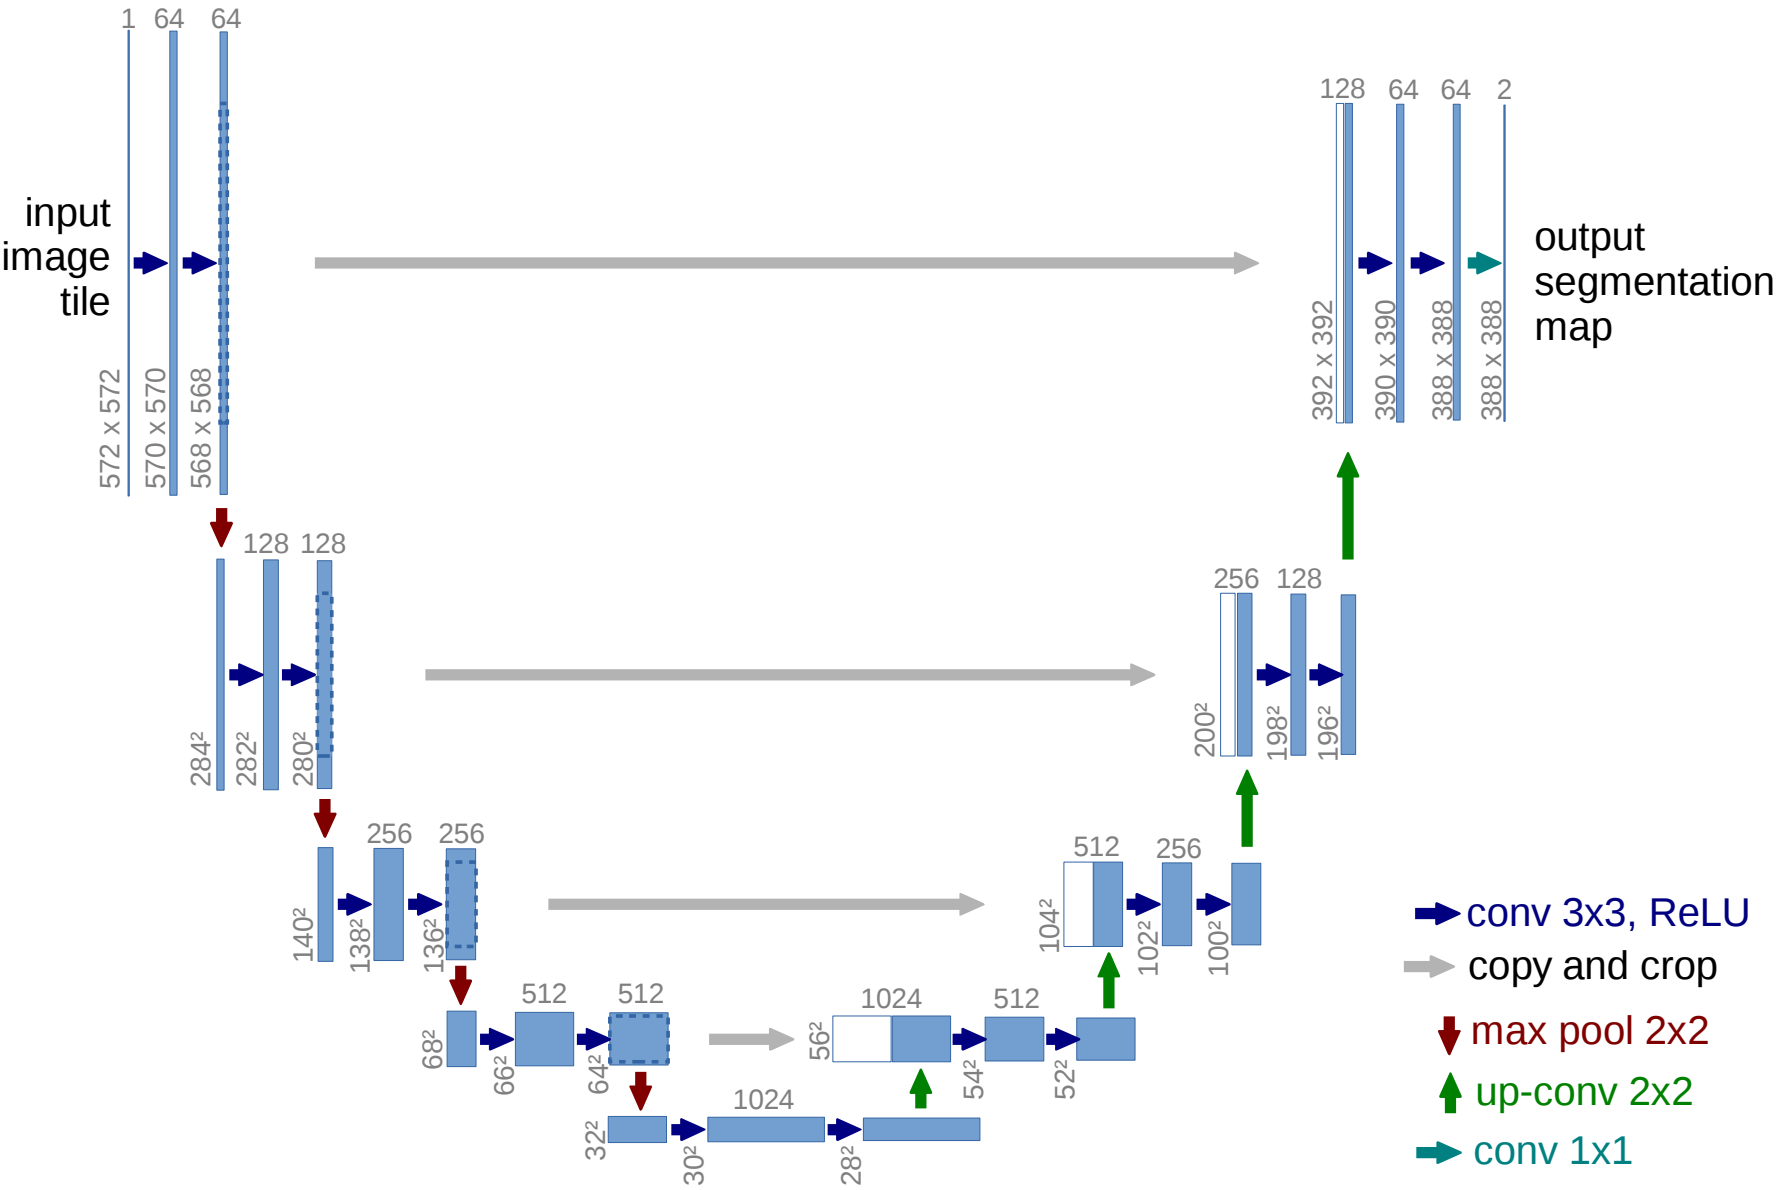
\includegraphics[width=0.48\columnwidth]{figs/unet.png}
\caption{Comparison of FCN and U-Net segmentation results.}
\label{fig:fcn_unet}
\end{figure}

\subsubsection{SegNet}
SegNet is a type of convolution neural network which uses encoder decoder architecture but focuses on computational efficiency and memory optimization \cite{badrinarayanan2016segnetdeepconvolutionalencoderdecoder}. The encoder used in this model is typically a classification network such as VGG \cite{badrinarayanan2016segnetdeepconvolutionalencoderdecoder}. It consists of multiple convolutional and pooling layers \cite{badrinarayanan2016segnetdeepconvolutionalencoderdecoder}. The model up-samples feature maps obtained from the encoder but does not use deconvolution filters \cite{badrinarayanan2016segnetdeepconvolutionalencoderdecoder}. This makes the model computationally efficient \cite{badrinarayanan2016segnetdeepconvolutionalencoderdecoder}. However, SegNet may not be a good choice for complex environments. This is because the model does not utilize skip connections.

\begin{figure*}[!t]
\centering
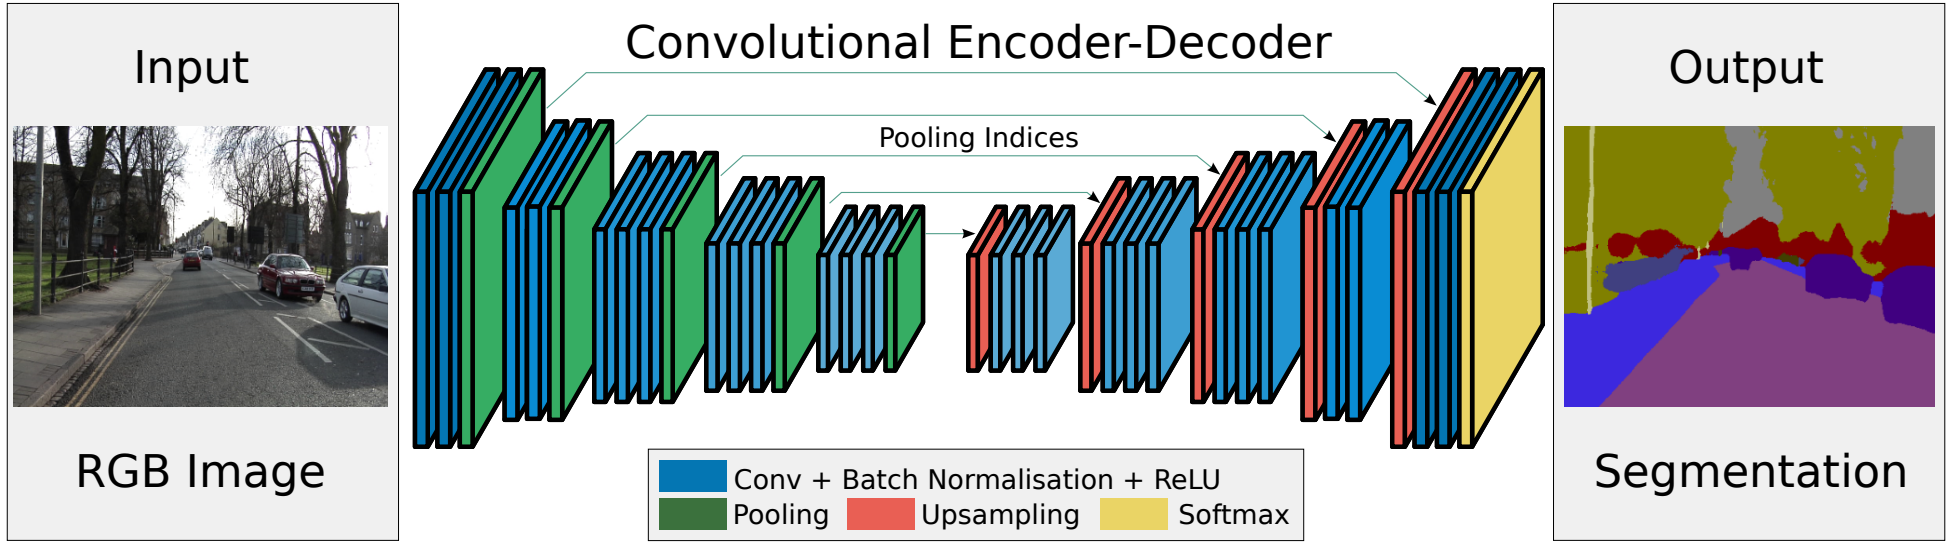
\includegraphics[width=0.48\textwidth]{figs/segnet.png}
\hfill
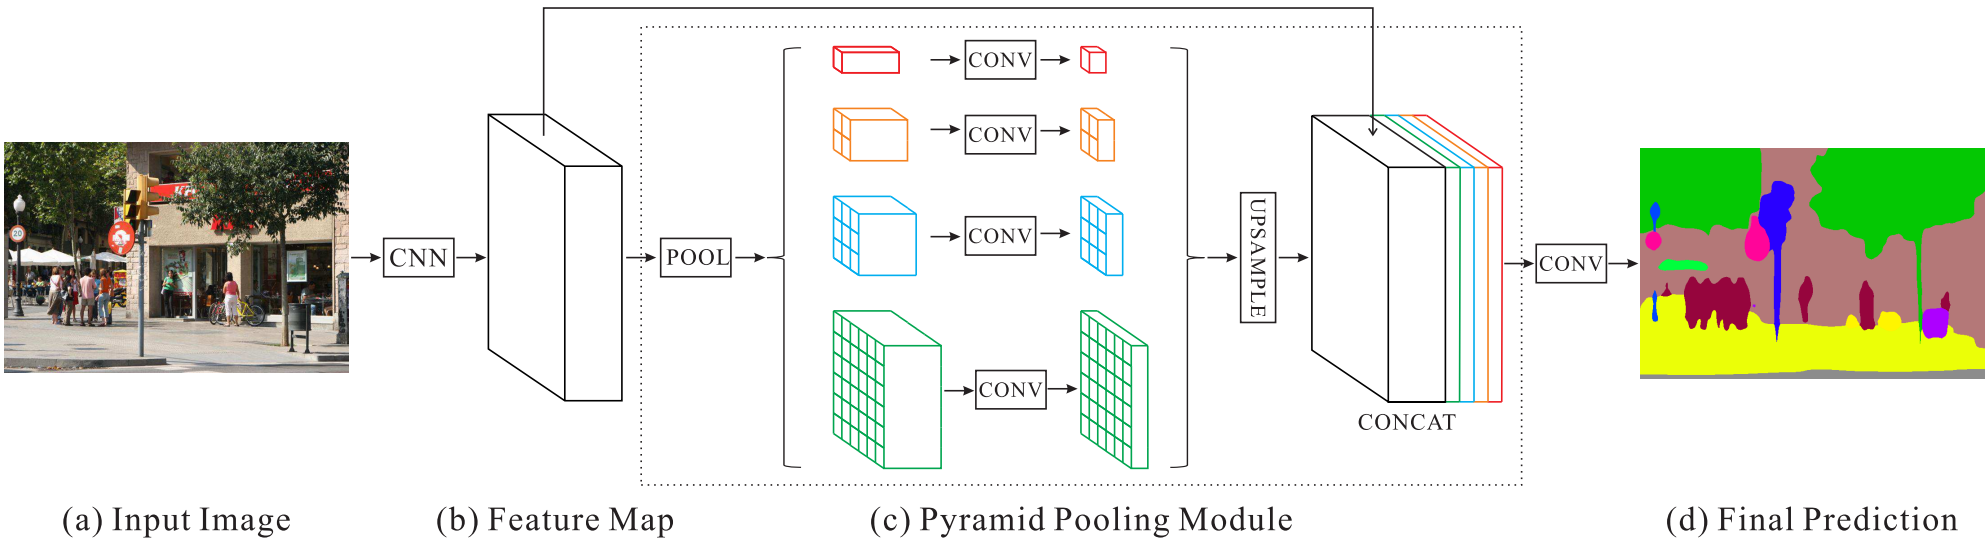
\includegraphics[width=0.48\textwidth]{figs/pspnet.png}
\caption{Examples of semantic segmentation using SegNet \cite{badrinarayanan2016segnetdeepconvolutionalencoderdecoder} and PSPNet \cite{zhao2017pyramidsceneparsingnetwork}.}
\label{fig:segnet_pspnet}
\end{figure*}

\subsubsection{DeepLabv3 and DeepLabv3+}
DeepLabv3 uses a new technique called atrous (dilated) convolutions to increase receptive field while controlling feature-map resolution \cite{chen2017rethinkingatrousconvolutionsemantic}. It also created a new technique called Atrous Spatial Pyramid Pooling (ASPP) to capture multi scale context through parallel artous rates \cite{chen2017rethinkingatrousconvolutionsemantic}. DeepLabv3+ is a newer iteration of the model which combines ASPP context encoding with an explicitly encoder decoder refinement path that joins low level features to sharpen boundaries \cite{chen2018encoder}. It also adds depthwise seperable convolutions to improve speed and accuracy tradeoffs \cite{chen2018encoder}.

\subsubsection{PSPNet}
Pyramid Scene Parsing Network (PSPNet) is a semantic segmentation model created to address the shorcoming of both FCNs and U-Net. It is created to capture global contexual information. FCN and U-Net may capture low-level to mid-level features well, it struggeles on incorporating scene-level understanding which is critical in complex environments \cite{zhao2017pyramidsceneparsingnetwork}. It uses Pyramid Pooling Module (PPM) that collects information at multiple spatial scales by applying pooling operations with different grid sizes over the feature map \cite{zhao2017pyramidsceneparsingnetwork}. These pooled features are upsampled again and concatenated with the original feature representations \cite{zhao2017pyramidsceneparsingnetwork}. This technique now allows the model to combine both global and local context to give more accurate predictions on pixel level \cite{zhao2017pyramidsceneparsingnetwork}. This exceptionally improved the perfomance and accuracry for objects with different sizes and relationships \cite{zhao2017pyramidsceneparsingnetwork}. This can be helpful for complex city images.

\subsubsection{SegFormer}
SegFormer is a modern semantic segmentation model whose architecure is based on transformers. It addresses limitations of previous convolutional models by capturing long-range dependencies and global context. It uses a transformer encoder called MiT – Mix Vision Transformer to take out multi-scale features without relying on positional encodings. This feature makes the model work well with varying input resolutions. This architecture uses a Multi Layered Perceptron (MLP) as a decoder to combine multi-level features from different stages of encoder to produce high-resolution segmentation maps. All of these techniques results in lower computational complexity while maintaining good performance.

\section{Benchmarking Results}
\subsection{Method Selection Criteria}
The models selected for this benchmarking test was FCN, DeepLabV3 and SegFormer. These models were chosen because it is very popular and has strong performance on datasets like Cityscapes and BDD100K. It is also computationally efficient and has architectural diversity. Its suitable for real time applications like Advanced Driver Assistance System (ADAS). These model will be able to show comparison between traditional deep learning segmentation models and modern transformer based segmentation models.

\subsection{Experimental Setup}
A qualitative and quantitative experimental benchmarking setup was done using sample images from both Cityscapes and BDD100K datasets. Cityscapes was used to test for structured urban street images while BDD100K was used to test real world driving conditions including nights and highways. Pretrained models from PyTorch and HuggingFace were used without training it manually due to system constraints. Each images of the two datasets were resized to the size of 512x512 and was processed using standard normalization. For each model qualitative performance was evaluated through visual segmentation output by mask overlays. The quantitative performance was evaluated through runtime average inference time (ms) and frames per second (FPS).

\begin{figure}[!t]
\centering
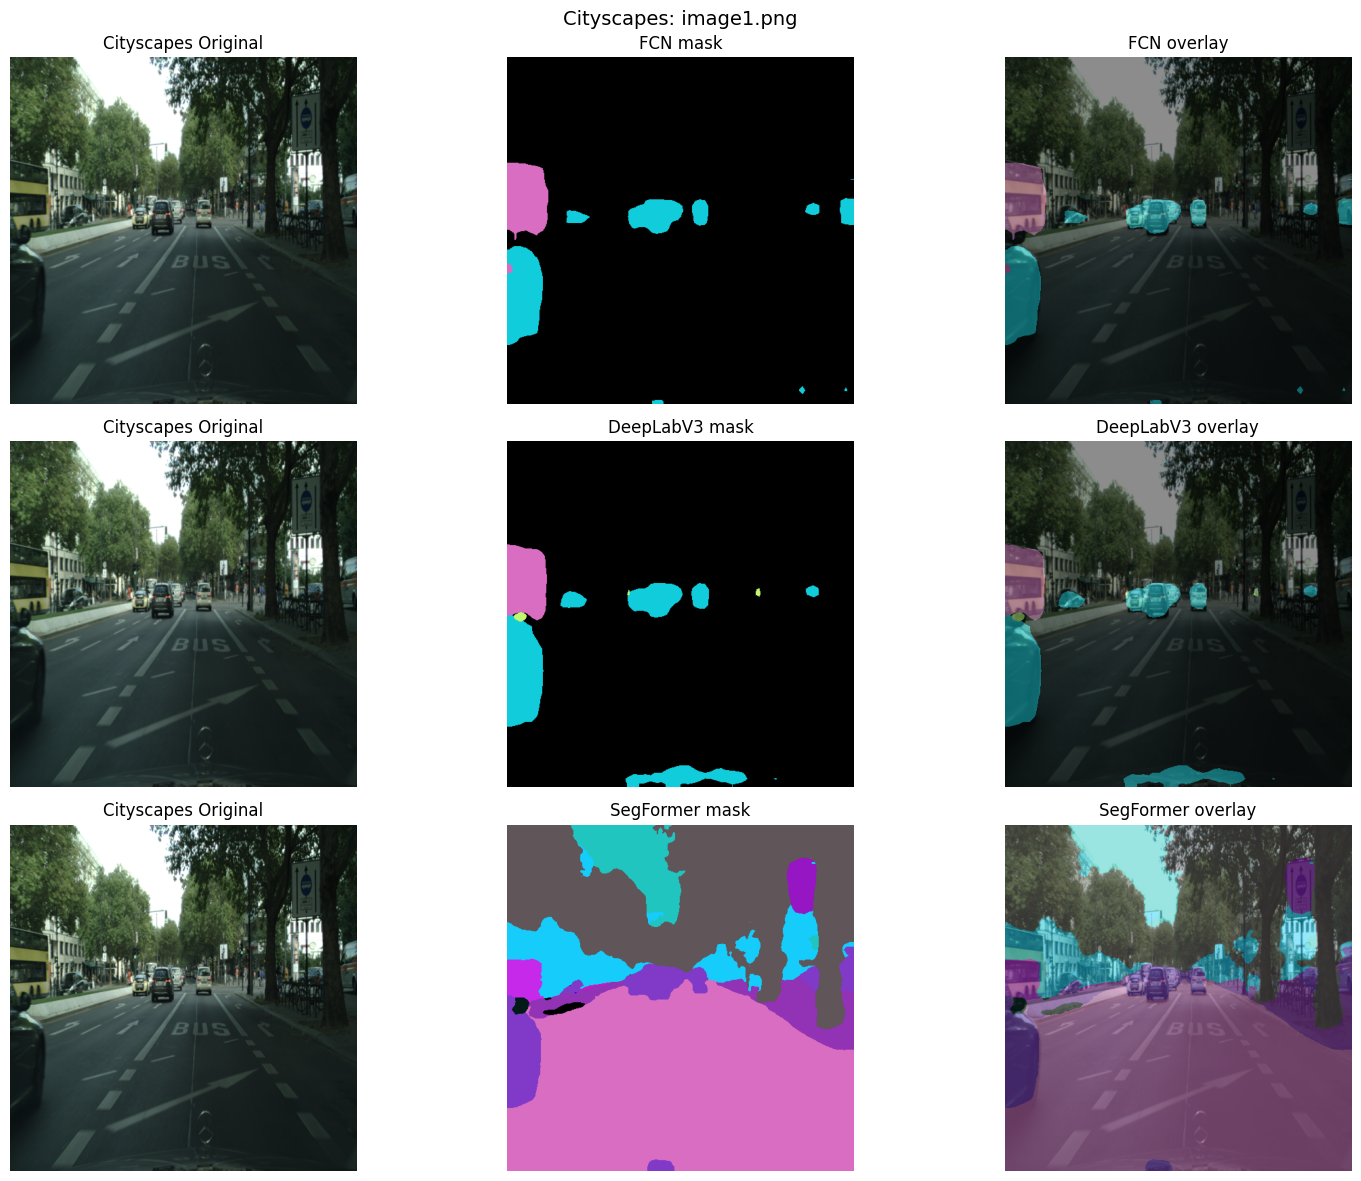
\includegraphics[width=\linewidth]{figs/comparision.png}
% where an .eps filename suffix will be assumed under latex, 
% and a .pdf suffix will be assumed for pdflatex; or what has been declared
% via \DeclareGraphicsExtensions.
\caption{Qualitative comparisons of segmentation models on Cityscapes dataset.}
\label{fig:comparision}
\end{figure}

\begin{figure}[!t]
\centering
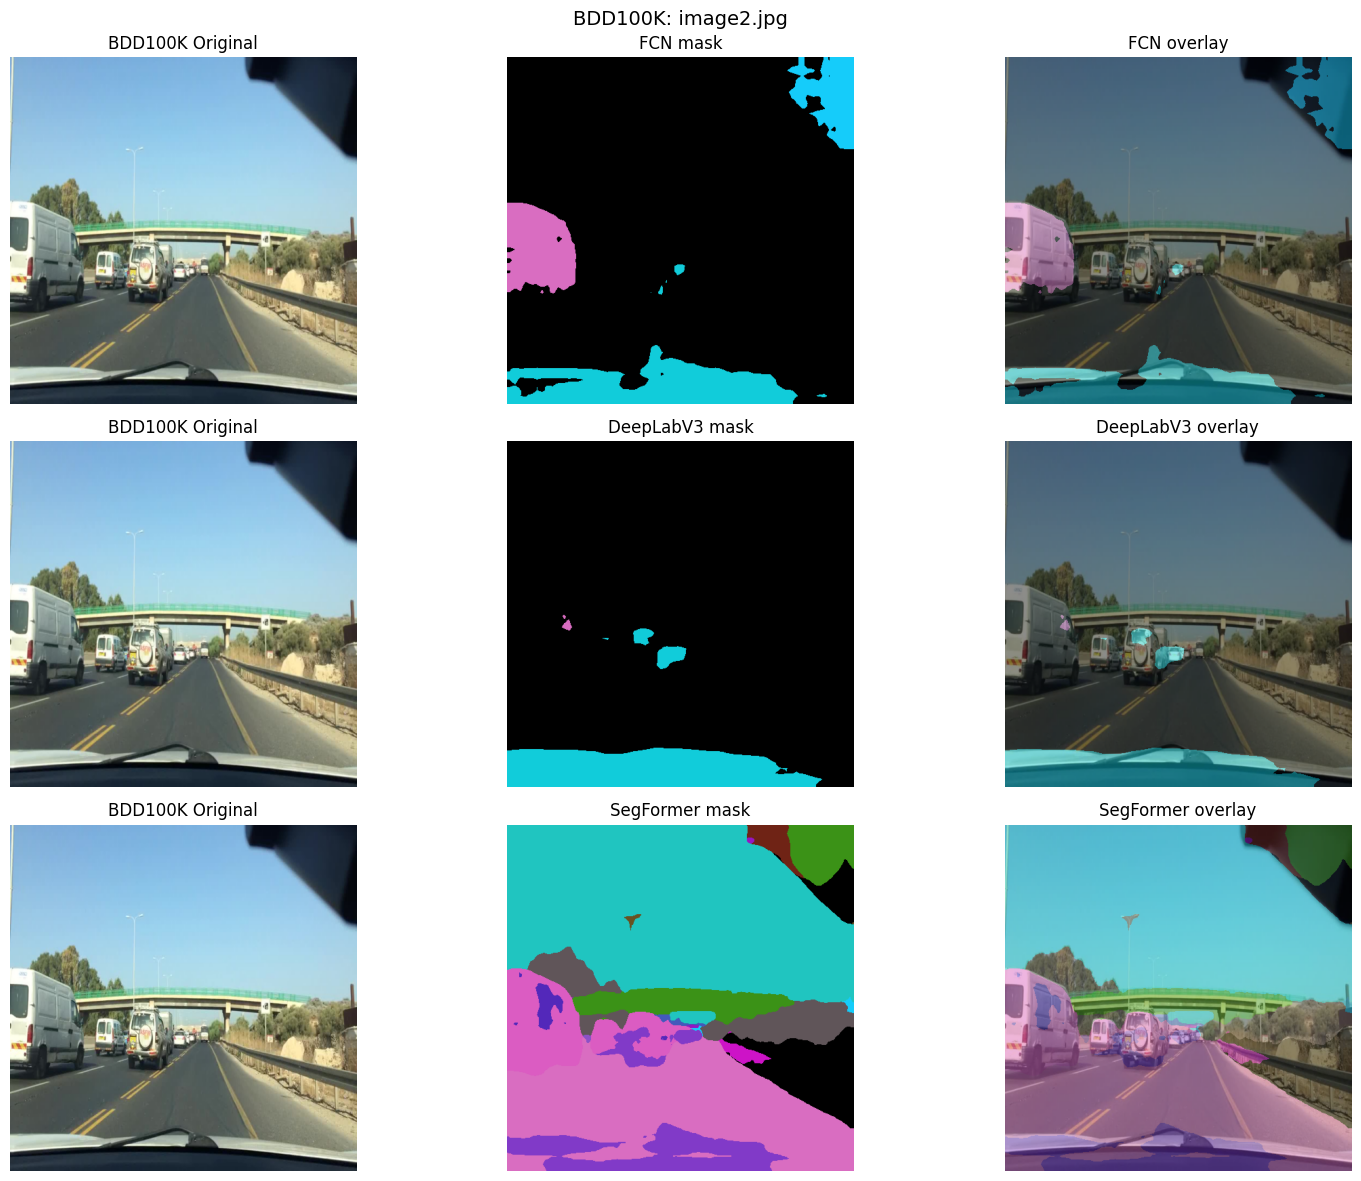
\includegraphics[width=\linewidth]{figs/comparision1.png}
\caption{Qualitative comparisons of segmentation models on BDD100K dataset.}
\label{fig:comparision1}
\end{figure}

\subsection{Qualitative Comparison}
Qualitative results show clear difference on the segmentation output of these models. From the visual outputs in Fig.~\ref{fig:comparision} and Fig.~\ref{fig:comparision1},, FCN produced coarse segmentation masks. It also struggled with object boundaries. It missed smaller objected in the image like smaller cars in distance. In comparison to DeepLabV3, it showed improvement from FCN in terms of object detection. It has better separation of vehicles, pedestrians and other smaller objects. It still produced fragmented masks in complex scenes as shown in Figure 5. SegFormer was the most consistent among the models. It produced dense segmentation masks. It captured both larger regions like road and sky, but also captured more smaller finer details. It also performed well under real world challenging conditions in BDD100K dataset. The images in the notebook file has also shown BDD100K performing well on SegFormer model. In BDD100K night images, SegFormer was successful in segmented larger regions like roads and surrounding environment. But, FCN and DeepLabV3 struggled detecting. It only detected limited object regions.

\subsubsection{Quantitative Benchmarking Results}
The runtime benchmarking results are given in Table~\ref{tab:inference_comparison}.
\begin{table}[!htbp]
\caption{Inference Performance Comparison on Cityscapes and BDD100K}
\centering
\begin{tabular}{|c|c|c|c|}
\hline
\textbf{Dataset} & \textbf{Model} & \textbf{Avg Inference Time (ms)} & \textbf{FPS} \\
\hline
Cityscapes & FCN       & 125.58 & 7.96  \\
Cityscapes & DeepLabV3 & 184.06 & 5.43  \\
Cityscapes & SegFormer & 60.36  & 16.57 \\
\hline
BDD100K    & FCN       & 119.80 & 8.35  \\
BDD100K    & DeepLabV3 & 170.07 & 5.88  \\
BDD100K    & SegFormer & 45.54  & 21.96 \\
\hline
\end{tabular}
\label{tab:inference_comparison}
\end{table}

The results show that SegFormer is the fastest model. It achieved lowest inference time and highest fps on both datasets. DeepLabV3 is the slowest model due to the artous convolution and multi-scale processing. FCN is the moderate option with moderate speed. It lacks accuracy when compared to other models.

\subsection{Comparative Analysis}
SegFormer was the most reliable segmentation model on both datasets. This was true in terms of complexity and low light scenarios in the environment of the image. DeepLabV3 had more accuracy over FCN due to its architecture. This was due to multi-scale context modeling. It still struggled on diverse environments. FCN showed limited capability in getting the finer minute details correct. This made it less suitable for applications. SegFormer also had highest real-time capable performance (16-22 FPS). This is suitable for deployment scenarios. DeepLabV3 had slower performance (5 FPS). This will limit the models' usability in real time systems. FCN model had acceptable speed but it lacked accuracy for real time systems. Across both datasets, all three models performed well on Cityscapes dataset. This may be true because the images are taken in structured environments. In BDK100K, the performance difference was seen drastically. This is due tot the dataset being more complex. FCN and DeepLabV3 had their performance degrade significantly. SegFormer maintained stable segmentation quality.

\subsection{Model Selection}
According the the results of benchmarking, SegFormer is the most suitable model for the problem. This is selected by the criteria of highest computational efficiency, strong qualitative performance, good performance in real world conditions and balance between accuracy and speed.

\section{Methodology}
The system uses a modular pipeline which consists of image input, preprocessing, benchmarking process and system implementation. The goal is to create a system that can be used as a driver assistance for heavy road freights in Australia. Input images are first standardized using normalization. It is then transformed to tensors and passed to given semantic segmentation models. The resulting output is then evaluated and benchmarked using various performance metrics. The system is implemented using the PyTorch deep learning framework. GPU acceleration was enabled during the process to improve inference performance.

Three semantic segmentation models were selected for the benchmarking process. These models were selected to each one of them represented different architectural approaches. The FCN was considered as the baseline convolutional model that performed pixel wise predictions by replacing fully connected layers with convolutional layers \cite{long2015fullyconvolutionalnetworkssemantic}. DeeplabV3 was selected as an advanced convolutional model because it used atrous convolutions and spatial pyramid pooling \cite{chen2018encoder}. SegFormer was chose because it represented different architecture through transformers. It is a transformer based model that used self attention mechanism to improve performance and accuracy. All of the images were converted to the size of 512x512 pixels to have consistency across models. There is a preprocessing pipeline which includes image resizing, converting to tensors, and normalization using mean and standard deviation. This normalization and standardization ensures compatibility with the pretrained models. There is also a benchmarking strategy to evaluate model performance. Each model goes through warm up phase to stabilize GPU performance. It is followed by multiple inference runs for measuring time. The warm up runs are done for five iterations. The benchmarking runs are done for twenty iterations. The GPU is also synchronized to ensure accurate timing measurements. The average inference time and frames per second (FPS) was then calculated. These metrics focus on computational efficiency. This is important for real time applications like autonomous driving systems.

The system was implemented using Pytorch with a machine equipped with NVIDIA GeForce GTX 1660 Ti GPU (6GB VRAM). CUDA acceleration was used to speed up the inference process. All of these models were run using evaluation mode. This disables the gradient computation to reduce memory overhead. Timing measurements were don using Python time module. GPU synchronization was done to ensure timing accuracy. To ensure the reproducibility of the system, these experiment process used a fixed processing pipeline and benchmarking protocol. This modular design enabled the system to allow easy integration of additional models or datasets. Also in terms of scalability, the system can also be extended to edge devices like Nvidia Jetson platforms by using optimized or quantized models. This makes the AI models run well offline and on resource constrained environments while maintaining reasonable performance.

\section{AI Ethics}
The Department of Industry, Science and Resources have published Australia's AI Ethics principles \cite{australia2019aiethics, dta2024transparency}. These principles are made for businesses and government bodies responsible in AI design, development and implementation. It focuses on improving safety, reliability, and fairness. It also helps in reducing negative impacts on people affected by AI. The principles applies in eight areas which include human, social and environmental well being; human-centered values; fairness; privacy protection and security; reliability and safety; transparency and explainability; contestability; and accountability \cite{australia2019aiethics, dta2024transparency}. In terms of road scenario segmentation context, the main benefits would be safety and accessibility. It will improve perception in drive assistance, and give hazard awareness. The camera in the system will capture images in public spaces. This can result in containing personal information. There is a need to treat these images as personal information under the privacy act \cite{australia2019aiethics}. There is also a need to implement a privacy by design. This means that following techniques of data minimization, shorter retention windows, strict access control, encryption and preprocessing that will reduce identification by blurring \cite{australia2019aiethics}.

\section{Discussion}
\subsection{United Nations Sustainable Development Goals}
The semantic segmentation system for road freight driver assistance system aligns with several goals from United Nations Sustainable Development Goals. (SDGs) \cite{UN_SDGs_2023}. 
\subsubsection{SDG 3: Good Health and Well-being}
Road accidents in heavy road freights is common in Australia. The use of driver assistance semantic segmentation models will improve the detection of hazards and objects like vehicles, animals, pedestrians, and lanes. This system will improve driver awareness by reducing human error. The system will then give safer road driving to drivers and reduce injuries an fatalities while driving.

\subsubsection{SDG 9: Industry, Innovation and Infrastructure}
The system uses advanced artificial intelligence models and techniques as its core function. This includes deep learning and transformer based models to improve transportation. Using these type of technology into freight vehicles is innovative. It helps in automation as well. This aligns on the goals focus on innovation and technological advancement.

\subsubsection{SDG 11: Sustainable Cities and Communities}
Proper, safe and efficient use of transportation systems is important for the safety and sustainability of cities and communities. The system helps in minimizing accidents and fatalities. This supports in sustainability.

\subsection{Carbon Footprint and Computational Efficiency}
The environmental aspect of AI systems is very important as  most AI system consume large amount of computational resources \cite{Arya2024}. This results in larger carbon footprint \cite{Arya2024}. The system in implementation is different in comparison to this. The system will use a pretrained SegFormer model. This model is lightweight and is capable of running on smaller system. The software will run on a edge device like Nvidia Jetson Nano or Nvidia Jetson AGX Orion. These are smaller edge device which operate on lower power. Since the system works on a edge device it will have almost none to low carbon footprint with extremely high computational efficiency.

\section{Conclusion}
This paper investigated the use of semantic segmentation techniques for improving perception in road freight driver-assistance system in Australia. The research focused on the evaluation and comparison of various models like FCN, DeepLabV3, SegFormer. The aim was to identify a model which worked best with the autonomous driving system. With the combination of literature review and benchmarking the study showed clear difference in the performance and accuracy between the models. Two datasets were used to evaluate these models and the result showed that SegFormer was better suited for real world deployment scenarios. The finding of this paper is important for Advanced Driver Assistance Systems (ADAS) in freight transport in Australia.

However, several limitations of this paper must be acknowledged. The benchmarking was done on a limited set of images with only two datasets. This is not effective for testing real world scenarios. The models were also pretrained and was not fine tuned which may affect performance in specific environments in Australia. In future work, large scale evaluations can be done using more finer tuned models and larger images and multiple datasets.

In conclusion, this study provides a comprehensive comparison and review of various semantic segmentation algorithms and models.





% if have a single appendix:
%\appendix[Proof of the Zonklar Equations]
% or
%\appendix  % for no appendix heading
% do not use \section anymore after \appendix, only \section*
% is possibly needed

% use appendices with more than one appendix
% then use \section to start each appendix
% you must declare a \section before using any
% \subsection or using \label (\appendices by itself
% starts a section numbered zero.)
%


\appendices
\section*{Appendix 1 - Video Presentation}
\begin{center}
    \url{https://echo360.net.au/media/8c5a1fef-d111-4d30-bb9f-5d9898eaa61e/public}
\end{center}

% you can choose not to have a title for an appendix
% if you want by leaving the argument blank
\section*{Appendix 2 -- Supplementary Materials}

\begin{center}
    \url{https://drive.google.com/drive/folders/1GoAjcK_MiVklquR_k9Z0XhL70XshVCXS?usp=sharing}
    \url{https://github.com/PrasannaTandukar/COMP6011}
\end{center}


% % use section* for acknowledgment
% \ifCLASSOPTIONcompsoc
%   % The Computer Society usually uses the plural form
%   \section*{Acknowledgments}
%   If you need to acknowledge anyone please include here.
% \else
%   % regular IEEE prefers the singular form
%   \section*{Acknowledgment}
% \fi





% Can use something like this to put references on a page
% by themselves when using endfloat and the captionsoff option.
\ifCLASSOPTIONcaptionsoff
  \newpage
\fi



% trigger a \newpage just before the given reference
% number - used to balance the columns on the last page
% adjust value as needed - may need to be readjusted if
% the document is modified later
%\IEEEtriggeratref{8}
% The "triggered" command can be changed if desired:
%\IEEEtriggercmd{\enlargethispage{-5in}}

% references section

% can use a bibliography generated by BibTeX as a .bbl file
% BibTeX documentation can be easily obtained at:
% http://mirror.ctan.org/biblio/bibtex/contrib/doc/
% The IEEEtran BibTeX style support page is at:
% http://www.michaelshell.org/tex/ieeetran/bibtex/
\bibliographystyle{IEEEtran}
\bibliography{references}


\end{document}


